\documentclass{article}
\usepackage[utf8]{inputenc}
\usepackage[T1]{fontenc}
\usepackage{lmodern}
\usepackage{amsmath, amssymb}
\usepackage{booktabs}
\usepackage{listings}
\usepackage{xcolor}
\usepackage{tikz}

\definecolor{codegray}{rgb}{0.4,0.4,0.4}
\definecolor{codepurple}{rgb}{0.58,0,0.82}
\definecolor{backcolour}{rgb}{0.95,0.95,0.92}

\lstdefinestyle{pythonstyle}{
  backgroundcolor=\color{backcolour},
  commentstyle=\color{codegray}\itshape,
  keywordstyle=\color{blue},
  numberstyle=\tiny\color{codegray},
  stringstyle=\color{codepurple},
  basicstyle=\ttfamily\small,
  breaklines=true,
  captionpos=b,
  keepspaces=true,
  numbers=left,
  numbersep=5pt,
  showspaces=false,
  showstringspaces=false,
  showtabs=false,
  language=Python
}

\title{Contrastive Loss: Fondamenti, Esempio e Diagnostica}
\author{Documentazione interna progetto \texttt{siamese}}
\date{\today}

\begin{document}

\maketitle

\section{Fondamenti teorici}
Una rete siamese $f_\theta : \mathcal{X} \rightarrow \mathbb{R}^d$ proietta ogni input $x$ in un vettore $z = f_\theta(x)$. Dato un insieme di coppie $\mathcal{D} = \{(x_i^a, x_i^b, y_i)\}_{i=1}^N$ con $y_i \in \{0,1\}$ (1 se la coppia è positiva, 0 altrimenti), la distanza euclidea tra gli embedding della coppia è
\[
  d_i = \|f_\theta(x_i^a) - f_\theta(x_i^b)\|_2.
\]

La contrastive loss classica \cite{hadsell2006dimensionality} assegna un costo individuale
\begin{equation}
  \mathcal{L}_i(\theta) = y_i\, d_i^2 + (1 - y_i)\, \max(0, m - d_i)^2,
  \label{eq:contrastive}
\end{equation}
con margin $m > 0$. Il valore globale è $\mathcal{L}(\theta) = \frac{1}{N} \sum_i \mathcal{L}_i(\theta)$.

\paragraph{Derivate.} Per $d_i > 0$, il termine gradiente sugli embedding della prima vista è
\begin{equation}
  \frac{\partial \mathcal{L}_i}{\partial z_i^a} =
  \begin{cases}
    2(z_i^a - z_i^b), & y_i = 1,\\[4pt]
    -2(m - d_i) \dfrac{z_i^a - z_i^b}{d_i}, & y_i = 0 \text{ e } d_i < m,\\[8pt]
    0, & y_i = 0 \text{ e } d_i \ge m,
  \end{cases}
  \label{eq:gradient}
\end{equation}
e simmetricamente per $z_i^b$. L'ottimizzatore discende lungo $-\nabla_\theta \mathcal{L}$ tramite la regola della catena
\[
  \frac{\partial \mathcal{L}}{\partial \theta} = \sum_{i=1}^N
  \left( \frac{\partial \mathcal{L}_i}{\partial z_i^a} \frac{\partial z_i^a}{\partial \theta}
  + \frac{\partial \mathcal{L}_i}{\partial z_i^b} \frac{\partial z_i^b}{\partial \theta} \right).
\]

\paragraph{Proprietà.} La loss è sempre non negativa ed è nulla quando tutte le coppie positive coincidono ($d_i = 0$) e tutte le coppie negative distano almeno $m$. Il termine di coppia negativa opera come vincolo di ``margine elastico'': una volta raggiunto $d_i \ge m$, la coppia smette di contribuire alla loss e quindi di fornire gradiente.

\begin{figure}[h]
  \centering
  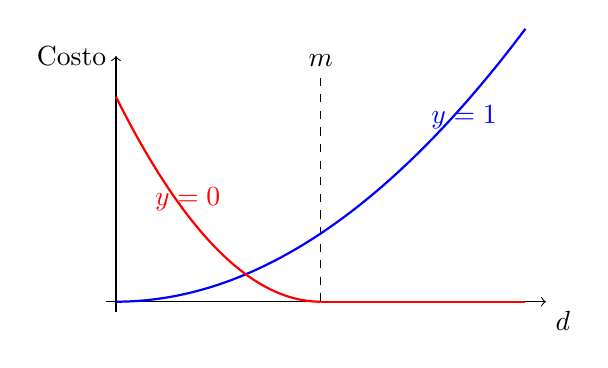
\begin{tikzpicture}[x=2.6cm, y=2.6cm]
    \draw[->] (-0.05,0) -- (2.1,0) node[below right]{$d$};
    \draw[->] (0,-0.05) -- (0,1.2) node[left]{Costo};
    \draw[dashed] (1,0) -- (1,1.1) node[above] {$m$};
    \draw[thick,blue,domain=0:2,samples=80] plot (\x, {\x*\x/3});
    \draw[thick,red,domain=0:1,samples=80] plot (\x, {(1-\x)^2});
    \draw[thick,red] (1,0) -- (2,0);
    \node[blue] at (1.7,0.9) {$y=1$};
    \node[red] at (0.35,0.5) {$y=0$};
  \end{tikzpicture}
  \caption{Forma dei termini della loss in funzione della distanza $d$ per margin $m=1$.}
  \label{fig:loss-shape}
\end{figure}

\section{Esempio concreto}
Consideriamo una rete lineare 2D $f_\theta(x) = Wx$, dove
\[
  W = \begin{pmatrix}
  1 & 0.2 & 0 \\
  0 & 0.8 & 0.4
  \end{pmatrix},
\]
e tre tipologie di segnali originari $x = (x_{\text{amp}}, x_{\text{freq}}, x_{\text{phase}}) \in \mathbb{R}^3$. Definiamo quattro campioni:
\[
\begin{aligned}
  a_1 &= (1.0, 0.9, 0.1), \quad &a_2 &= (0.8, 1.1, 0.2),\\
  b_1 &= (2.1, 1.9, 0.4), \quad &c_1 &= (2.0, 0.4, 1.2).
\end{aligned}
\]
I primi due appartengono alla stessa classe, mentre $b_1$ e $c_1$ rappresentano classi differenti.

\subsection*{Embedding e distanze}
Calcoliamo gli embedding:
\[
  f_\theta(a_1) = (1.18,\,0.76), \quad
  f_\theta(a_2) = (1.02,\,0.96), \quad
  f_\theta(b_1) = (2.48,\,1.68), \quad
  f_\theta(c_1) = (2.08,\,0.80).
\]

Le distanze euclidee diventano:
\[
\begin{aligned}
  d_{\text{pos}} &= \|f_\theta(a_1) - f_\theta(a_2)\|_2 \approx 0.256,\\
  d_{ab} &= \|f_\theta(a_1) - f_\theta(b_1)\|_2 \approx 1.593,\\
  d_{ac} &= \|f_\theta(a_1) - f_\theta(c_1)\|_2 \approx 0.901.
\end{aligned}
\]
Con margin $m = 1.0$ otteniamo i contributi:
\[
\begin{aligned}
  \mathcal{L}_{\text{pos}} &= d_{\text{pos}}^2 \approx 0.0656,\\
  \mathcal{L}_{ab} &= 0 \quad (\text{coppia negativa oltre il margin}),\\
  \mathcal{L}_{ac} &= (m - d_{ac})^2 \approx 0.0098.
\end{aligned}
\]
Il batch presenta quindi un termine dominante dalla coppia positiva e un termine negativo molto più piccolo ma non nullo, che continuerà a spingere $c_1$ lontano da $a_1$ finché la distanza non supera stabilmente il margin.

\subsection*{Gradiente indotto dai termini di loss}
Per comprendere come lo scalare $\mathcal{L}_i$ orienti gli aggiornamenti, valutiamo il gradiente rispetto all'embedding $z(a_1)$ sfruttando \eqref{eq:gradient}.
\begin{itemize}
  \item \textbf{Coppia positiva $(a_1,a_2)$.} La differenza degli embedding è $z(a_1) - z(a_2) = (0.16, -0.20)$. Il gradiente è quindi
  \[
    \frac{\partial \mathcal{L}_{\text{pos}}}{\partial z(a_1)} = 2(z(a_1) - z(a_2)) = (0.32,\,-0.40),
  \]
  vettore che punta direttamente da $z(a_1)$ verso $z(a_2)$ e spinge i due punti a coincidere.
  \item \textbf{Coppia negativa attiva $(a_1,c_1)$.} Poiché $d_{ac} < m$, il gradiente vale
  \[
    \frac{\partial \mathcal{L}_{ac}}{\partial z(a_1)} = -2 (m - d_{ac}) \frac{z(a_1) - z(c_1)}{d_{ac}}.
  \]
  Con $z(a_1) - z(c_1) = (-0.90,-0.04)$ otteniamo
  \[
    \frac{\partial \mathcal{L}_{ac}}{\partial z(a_1)} \approx (0.198,\,0.009),
  \]
  direzione che spinge $z(a_1)$ lontano da $z(c_1)$ lungo la congiungente.
  \item \textbf{Coppia negativa inattiva $(a_1,b_1)$.} Poiché $d_{ab} > m$, il termine è nullo e non produce gradiente.
\end{itemize}
Il gradiente totale su $z(a_1)$ è la somma dei contributi attivi: un vettore che combina una forte attrazione verso $a_2$ e una debole repulsione da $c_1$. L'ottimizzatore trasmette quindi queste spinte ai parametri $\theta$ tramite la regola della catena, pur partendo da una loss che è un singolo scalare aggregato.
Tutti i valori numerici sono riproducibili eseguendo lo script \texttt{docs/contrastive\_example\_gradients.py}.

\section{Diagnostica del collasso delle distanze}
\subsection*{Fenomeno}
In alcune configurazioni gli embedding tendono a ridurre la loro norma complessiva, facendo collassare sia le distanze intra-classe sia quelle inter-classe verso zero. La loss può comunque diminuire perché il rapporto tra le due rimane favorevole, ma la separazione assoluta perde significato metrico.

\subsection*{Cause comuni}
\begin{itemize}
  \item Margin troppo piccolo: le coppie negative escono rapidamente dalla zona attiva e non forniscono più gradiente repulsivo.
  \item Campionamento di coppie poco informative: se i batch contengono soprattutto esempi facili, i gradienti negativi si esauriscono presto.
  \item Regolarizzazioni o bias architetturali che riducono sistematicamente la norma degli embedding (weight decay elevato, normalizzazioni aggressive, attivazioni sature).
  \item Dati sovrapposti o rumorosi: separare davvero costa più che comprimere uniformemente gli embedding.
\end{itemize}

\subsection*{Contromisure}
\begin{itemize}
  \item Aumentare il margin o adattarlo dinamicamente per mantenere attivo un numero significativo di coppie negative.
  \item Implementare hard/semi-hard negative mining o una strategia di sampling che garantisca varietà intra-batch.
  \item Monitorare e regolarizzare la norma degli embedding (ad esempio con L2 normalization seguita da scaling controllato o con un termine di center loss).
  \item Passare temporaneamente a loss che penalizzano il collasso (Triplet, Circle Loss, InfoNCE) per re-iniettare separazione assoluta.
\end{itemize}

Queste osservazioni chiudono il cerchio tra descrizione teorica e comportamento empirico, evidenziando come la struttura della loss imponga condizioni sufficienti ma non necessarie per mantenere distanze assolute elevate.

\bibliographystyle{plain}
\begin{thebibliography}{1}
\bibitem{hadsell2006dimensionality}
R.~Hadsell, S.~Chopra e Y.~LeCun.
\newblock Dimensionality Reduction by Learning an Invariant Mapping.
\newblock In \emph{CVPR}, 2006.
\end{thebibliography}

\end{document}
